\newcommand{\ox}{\overline x}

\chapter[Integración numérica]{Integración numérica%
\footnote{\licenseInfo}}
\label{cha:integracion-numerica}

El cálculo de una integral definida es un problema que aparece con
frecuencia, tanto en matemáticas como en otro ámbitos (ciencia,
ingeniería, economía,...). En concreto, dada una función
$f:[a,b]\subset\Rset\to\Rset$, se trata de aproximar numéricamente su
integral definida en $[a,b]$,
\begin{equation*}
  \int_a^bf(x)\,dx.
\end{equation*}

La necesidad de la aproximación numérica de integrales definidas
estriba en que, con frecuencia, resulta imposible (o demasiado costoso
computacionalmente) su cálculo de forma exacta. No sólo porque, en
contextos experimentales, la función podría venir dada por una tabla
de datos, sino porque la mayor parte de las funciones matemáticas no
son integrables mediante las técnicas usuales del cálculo elemental
y por tanto no resulta aplicable la regla de Barrow, $\int_a^b f(x)\,
dx=F(b)-F(a)$.

En este tema se plantearán métodos o fórmulas numéricas, llamadas
fórmulas de cuadratura, para la aproximación de $\int_a^b f(x)\,
dx$. La primera idea es la sustitución de $f(x)$ por un interpolador,
$p_n(x)$, de forma que $\int_a^bf(x)\,dx \approx \int_a^b p_n(x)\,
dx$. Esta última integral es fácil de calcular y, como veremos,
expresar como $\sum_{i=0}^n \omega_i \, f(x_i)$ (donde los coeficiente
$\omega_i$ provienen, por ejemplo, de la integración de las
funciones base de Lagrange).


Por tanto, las fórmulas de cuadratura para la aproximación de
$\int_a^b f(x)\, dx$ serán expresiones que utilizan los valores de la
función en un conjunto de $n+1$ \emph{nodos}, $\{x_0,x_1,\dots,x_n\}$,
multiplicados por $n+1$ \emph{pesos}
$\{\omega_0,\omega_1,\dots,\omega_n\}$:
\begin{definition}[Fórmula de cuadratura de tipo general]
  \label{def:formula-cuadratura}
  Una \resaltar{fórmula de cuadratura} (abreviadamente, f.c.) con
  $n+1$ nodos $\{x_i\}_{i=0}^n$ y pesos $\{\omega_i\}_{i=0}^n$ es una
  expresión del tipo:
  \begin{align}
    \label{eq:f.cuadratura}
    I_n(f)&=\sum_{i=0}^n \omega_i \, f(x_i).
    \\
    \intertext{Al valor}
    \notag
    E_n(f) &= \int_a^b f(x) - I_n(f) 
  \end{align}
  se le llama \resaltar{error} de la fórmula de cuadratura (o
  simplemente \resaltar{error de cuadratura} o error de integración). 
  % donde $I_n(f)\in\Rset$ representa un valor aproximado de $\int_a^b
  % f(x)\,dx$ y $E_n(f)\in\Rset$ es el error que se comete en la
  % aproximación.
\end{definition}
Indicando que el error <<será pequeño>>, escribimos:
\begin{equation*}
  I_n(f) \approx \int_a^b f(x)\, dx.
\end{equation*}

\begin{definition}[Orden de una fórmula de cuadratura]
  \label{def:2}
  Una fórmula de cuadratura se dirá de \resaltar{orden} $m\in\Nset$ si
  verifica:
  \begin{align*}
    E_n(p)&=0 \quad \forall p\in\Pol_m[x] \text{ (polinomios
      de grado menor o igual que $m$) y}
    \\
    E_n(p)&\neq 0 \quad \text{para \emph{algún} polinomio }
    p\in\Pol_{m+1}[x] \text{ (de grado $m+1$)}.
  \end{align*}
\end{definition}
Así, decimos que una fórmula de cuadratura de orden $m$ es exacta para
los polinomios de orden (menor o igual a) $m$, pero no para los de
orden $m+1$.
\begin{remark}
  \label{rk:5}
  Utilizando la linealidad con respecto a $f$ de $\int_a^bf(x)\,dx$ y
  de $I_n(f)$, es evidente que una f.c. es de orden $m\in\Nset$ si
  y sólo si verifica:
  \begin{align*}
    E_n(x^k)&=0 \quad \forall k=0\dots,m \text{ y}
    \\
    E_n(x^{m+1})&\neq 0.
  \end{align*}
  Esta suele ser la forma de estudiar, en la práctica, el orden de una
  fórmula de cuadratura.
\end{remark}

\begin{example}
  \label{ex:formula-punto-medio}
  La siguiente fórmula de cuadratura de un punto ($n=0$) es conocida
  como \resaltar{fórmula del punto medio},
  \begin{equation}
    \label{eq:f.c.-pto-medio}
    I_0(f)= (b-a) f\left(\frac{a+b}{2}\right),
  \end{equation}
  y tiene orden $1$. En efecto, evaluando $E_0(x^k)=\int_a^b
  x^k\, dx-I_0(x^k)$ para $k\ge 0$:
  \begin{align*}
   \text{Para } k&=0:\ E_0(1) = \int_a^b 1\cdot dx - (b-a)\cdot 1 = 0.
   \\
   \text{Para } k&=1:\ E_0(x) = \int_a^b x\cdot dx - (b-a)\frac{a+b}{2}
   = \frac{1}{2}(b^2-a^2) -  (b-a) \frac{a+b}{2} = 0.
   \\
   \text{Para } k&=2:\ E_0(x^2) = \int_a^b x^2\cdot dx 
   - (b-a) \frac{(a+b)^2}{4} 
   = \frac{1}{3}(b^3-a^3) - (b-a)\frac{(a+b)^2}{4} 
   \neq 0.
  \end{align*}
\end{example}

\begin{example}
  \label{ex:formula-trapecio}
  La siguiente f.c. de dos puntos ($n=1$) es conocida
  como \resaltar{fórmula del trapecio}:
  \begin{equation*}
    I_1(f)= \frac{b-a}{2}\left(f(a)+f(b)\right).
  \end{equation*}
  La formula del trapecio es de orden 1:
  \begin{align*}
    \text{Para } k&=0:\ E_1(1) = (b-a) - \frac{b-a}2\cdot 2 = 0.
    \\
    \text{Para } k&=1:\ E_1(x) = \frac{b^2-a^2}{2} -
    \frac{(b-a)}{2}(a+b) = 0.
    \\
    \text{Para } k&=2:\ E_1(x^2) = \frac{b^3-a^3}{3} -
    \frac{(b-a)}{2}(a^2+b^2) \neq 0.
  \end{align*}
\end{example}

\begin{example}
  \label{ex:formula-simpson}
  La \resaltar{fórmula de Simpson} es la siguiente f.c.
  de tres puntos ($n=2$):
  \begin{equation}
    I_2(f)= \frac{b-a}{6}\left[f(a)+4f
      \left(\frac{a+b}{2}\right)+f(b)\right].
    \label{eq:formula-simpson}
  \end{equation}
  Su orden es $3$. La demostración es similar a los ejemplos anteriores.
\end{example}

\section{Fórmulas de cuadratura de tipo interpolatorio}
\label{sec:cuadratura-interpolatorio}

La expresión~(\ref{eq:f.cuadratura}) define a una fórmula de
cuadratura de tipo general, para pesos $\omega_i$ y nodos $x_i$
cualesquiera, no necesariamente provenientes de la interpolación.
Pero por motivos que veremos luego
(proposición~\ref{pro:existencia.fcti}), nos interesarán especialmente
aquellas fórmulas de cuadratura que vengan dadas por integración de un
polinomio de interpolación.
\begin{definition}[Fórmula de cuadratura de tipo interpolatorio]
  Sea $f\in C^0([a,b])$ y sea $p_n$ el polinomio de interpolación de
  Lagrange asociado a $f$ y a $n+1$ nodos
  $\{x_0,x_1,\dots,x_n\}$. Diremos que una f.c. es de tipo
  interpolatorio si 
  \begin{equation}
    \label{eq:fcti}
    I_n(f)=\int_a^b p_n(x)\, dx.
  \end{equation}
  \label{def:fcti}
\end{definition}

La expresión~(\ref{eq:fcti}) se puede escribir de la forma
de~(\ref{eq:f.cuadratura}), es decir como suma de $f(x_i)$ por
cierto pesos. En efecto, dada $f\in C^0([a,b])$, podemos escribir
$p_n$ usando la fórmula de interpolación de Lagrange:
\begin{equation*}
  p_n(x)=\sum_{i=0}^n f(x_i) L_i(x),
\end{equation*}
donde $\{L_i\}_{i=0}^n$ es la base de Lagrange asociada a
$\{x_i\}_{i=0}^n$. Por lo tanto,
\begin{equation*}
  \int_a^bp_n(x)\,dx = \sum_{i=0}^n f(x_i) \int_a^b L_i(x)\,dx 
  =\sum_{i=0}^n \omega_i f(x_i), \quad \text{con } \omega_i=\int_a^b L_i(x)\,dx.
\end{equation*}

\begin{example}
  \label{ex:formula-pto-medio-interpol}
  La f.c. del punto medio~(\ref{eq:f.c.-pto-medio}) es de tipo
  interpolatorio. En efecto, si $p_0(x)$ es el polinomio de 
  interpolación de grado cero asociado a $f$ en $x_0=(a+b)/2$, es
  decir $p_0(x)=f(x_0)$ para todo $x\in[a,b]$, entonces:
  \begin{equation*}
    I_0(f) = (b-a)f\left(\frac{a+b}{2}\right) = \int_a^b p_0(x)\,dx.
  \end{equation*}
\end{example}

\begin{example}
  \label{ex:formula-trapecio-interpol}
  Fijamos $n=1$, $x_0=a$ y $x_1=b$. Buscamos coeficientes, $\omega_0$
  y $\omega_1$ tales que la siguiente fórmula de cuadratura sea de
  tipo interpolatorio:
  \begin{equation*}
    I_1(f)=\omega_0 f(x_0) + \omega_1 f(x_1).
  \end{equation*}
  Según la definición~\ref{def:fcti}, esto significa que
  \begin{equation*}
    I_1(f)=\int_a^b p_n(x)= 
    \underbrace{\left(\int_a^bL_0(x)\right)}_{\omega_0} f(x_0)+
    \underbrace{\left(\int_a^bL_1(x)\right)}_{\omega_1} f(x_1).
  \end{equation*}
  Como
  \begin{equation*}
    L_0(x)=\frac{x-x_1}{x_0-x_1}=\frac{x-b}{a-b} \quad \text{y} \quad
    L_1(x)=\frac{x-x_0}{x_1-x_0}=\frac{x-a}{b-a},
  \end{equation*}
  entonces
  \begin{equation*}
    \omega_0 = \int_a^b \frac{x-b}{a-b} = \frac{-(a-b)^2}{2(a-b)}=\frac{b-a}{2},
    \quad
    \omega_1 = \int_a^b \frac{x-a}{b-a} = \frac{(b-a)^2}{2(b-a)}=\frac{b-a}{2}.
  \end{equation*}
  Es decir, que la fórmula de cuadratura que buscamos es la
  fórmula del trapecio:
  \begin{equation*}
    I_1(f)=\frac{b-a}{2}
    \left(
      f(a)+f(b)
    \right).
  \end{equation*}
\end{example}

\begin{example}
  La fórmula de Simpson~(\ref{eq:formula-simpson}) es de tipo
  interpolatorio. La demostración se deja como ejercicio.
\end{example}

La siguiente proposición afirma que las f.c.t.i. son óptimas, en el
sentido de que son las f.c. de mayor orden.
\begin{proposition}
  \label{pro:existencia.fcti}
  Dados $n+1$ nodos distintos, $x_0<x_1<\cdots<x_n$:
  \begin{enumerate}
  \item Sobre estos nodos existe una única f.c. con orden $\ge
    n$.
  \item Esta f.c. coincide con la f.c.t.i. correspondiente a
    $\{x_i\}_{i=0}^n$.
  \end{enumerate}
\end{proposition}
\begin{proof}~\par
  \punto{1} Sea $I_n(f)=\sum_{i=0}^n \omega_i f(x_i)$ una
  f.c. cualquiera sobre $\{x_i\}_{i=0}^n$. $I_n(f)$ tiene orden $\ge
  n$ si y solo si $E(x^k)=0$ para $k=0,\dots,n$. Escribiendo estas $n+1$
  ecuaciones,
  \begin{equation}
    \left.
  \begin{alignedat}{2} % 2 bloques de columnas rl
    E(1)&=0 \quad \Leftrightarrow\ \quad &
    \omega_0 + \omega_1 + \cdots \omega_n &=
    \int_a^b 1\cdot\,dx = b-a
    \\
    E(x)&=0 \quad \Leftrightarrow\ \quad &
    \omega_0 x_0 + \omega_1 x_1 + \cdots \omega_n x_n &=
    \int_a^b x \cdot\,dx = \frac{b^2-a^2}{2}
    \\
    &\ \, \vdots & &\ \, \vdots
    \\
    E(x^n)&=0 \quad \Leftrightarrow\ \quad &
    \omega_0 x_0^n + \omega_1 x_1^n + \cdots \omega_n x_n^n &=
    \int_a^b x^n \cdot\,dx = \frac{b^{n+1}-a^{n+1}}{n+1}
    \\
  \end{alignedat}
  \right\}
  \label{eq:sl.fcti}
\end{equation}
  tenemos un sistema lineal con $n+1$ incógnitas
  $\{\omega_i\}_{i=0}^n$. La matriz asociada, es la conocida matriz de
  Vandermonde, 
  \begin{equation*}
    A =
    \begin{pmatrix}
      1 & x_0& \cdots & x_0^n \\
      1 & x_1& \cdots & x_1^n \\
      \vdots & \vdots & & \vdots \\
      1 & x_n& \cdots & x_n^n 
    \end{pmatrix}
  \end{equation*}
  que fue estudiada en el teorema~\ref{thm:existencia-unicidad-lagrange}
  (existencia y unicidad del polinomio de interpolación de Lagrange),
  donde comprobamos que $A$ no es singular si los nodos son distintos.
  Por lo tanto, existe una única solución, $\{\omega_i\}_{i=0}^n$, que
  determina la única f.c. $I_n(f)$ de orden $\ge n$.

  \punto{2} Veamos que esta única f.c. de orden $\ge n$ coincide con
  la f.c.t.i. correspondiente a $\{x_i\}_{i=0}^n$. Para ello, basta
  comprobar que la f.c.t.i. definida sobre nodos $\{x_i\}_{i=0}^n$
  tiene orden al menos $n$. 
  Pero esto es evidente: sea $I_n(f)=\int_a^b p_n(x)\, dx$ donde $p_n$
  interpola a $f$ en los nodos $\{x_i\}_{i=0}^n$. Si $f(x)=p(x)$ es un
  polinomio de grado $\le n$, entonces su polinomio de interpolación
  de Lagrange es $p_n(x)=p(x)$ (por unicidad), por tanto
  $E_n(p)=\int_a^b p(x)\,dx - \int_a^b p_n(x)\,dx =0$.
\end{proof}

\begin{remark}
  \label{rk:6}
  La demostración de la proposición anterior nos proporciona una forma
  de calcular los pesos de cualquier f.c.t.i.: resolver el sistema
lineal~(\ref{eq:sl.fcti}). Este método se conoce como \resaltar{método de
  los coeficientes indeterminados}. Tiene el inconveniente de que su
matriz asociada, la matriz de Vandermonde, está mal condicionada
  cuando $n\to\infty$.
\end{remark}

\begin{example}
  \label{ex:coef-indetermin:formula-trapecios-abierta}
  Utilizaremos el método de los coeficientes indeterminados para
  calcular los pesos de la fórmula de cuadratura en $[a,b]$ que es de
  mayor orden (es decir, la f.c.t.i.) para los nodos $x_0=a+h$ y
  $x_1=a+2h$, con $h=\frac{b-a}{3}$.
  
  Para $n=1$, obtenemos el siguiente sistema:
  \begin{align*}
    \omega_0 + \omega_1 &= b-a,
    \\ 
    x_0\omega_0 + x_1\omega_1 &= \frac{b^2-a^2}{2},
  \end{align*}
  cuya única solución es:
  \begin{equation*}
    \omega_0=\omega_1=\frac{3h}{2}
  \end{equation*}
  Así obtenemos la siguiente fórmula de cuadratura (que es conocida
  como \textit{fórmula de los trapecios abierta}:
  \begin{equation*}
    I_1(f)=\frac{3h}{2}
    \left(
      f(x_0)+f(x_1),
    \right)
    \quad \text{con } x_0=a+h, \ x_1=a+2h,
  \end{equation*}
  para $h=\frac{b-a}{3}$.
\end{example}

\subsection*{Cota del error en fórmulas de tipo interpolatorio}

Sea $I_n(f)$ una f.c.t.i. sobre $n+1$ puntos y sea $p_n$ el polinomio
de Lagrange asociado.  Utilizando la
expresión~(\ref{eq:expresion-error-interpol}) de error de
interpolación del polinomio de Lagrange podemos razonar como sigue:

\begin{align*}
  E_n(f)=&\int_a^b f(x)\, dx - I_n(f) =
  \int_a^b\left(f(x)-p_n(x)\right)\,dx 
  \\
  =&\int_a^b \frac{f^{n+1)}(\xi_x)}{(n+1)!} (x-x_0)(x-x_1)\dots(x-x_n) \,dx
  \le \int_a^b  \frac{M_{n+1}}{(n+1)!} (b-a)^{n+1} \, dx,
\end{align*}
donde $M_{n+1}=\max_{x\in [a,b]} |f^{n+1)}(x)|$.
Por lo tanto toda f.c.t.i con $n+1$ puntos en un intervalo $[a,b]$
verifica la siguiente cota del error:
\begin{equation}
  E_n(f) \le  \frac{M_{n+1}}{(n+1)!} (b-a)^{n+2}y.
  \label{eq:cota-error-fcti}
\end{equation}

Tal y como en el capítulo~\ref{cha:Interpolacion-aproximacion}, nos
podemos preguntar: dada una f.c.t.i., para una función $f$
suficientemente regular (por ejemplo infinitamente derivable),
¿podemos garantizar que $E_n(f)$ tiende a cero cuando $n\to\infty$?,
es decir,
\begin{eqnarray*}
  \text{\large ¿ \;} 
  \lim_{n\to\infty} \int_a^b p_n(x) = \int_a^bf(x)
  \text{\; \large?}
  \label{eq:pregunta.p_n.to.f}
\end{eqnarray*}
Una vez más, la respuesta a esta pregunta es negativa, en general, como
sugiere el hecho de que en la estimación~(\ref{eq:cota-error-fcti}) no
resulta posible acotar el término $M_{n+1}$, para cualquier función
infinitamente derivable, cuando $n\to\infty$.

Sin embargo, si denotamos el tamaño del intervalo como $h=(b-a)$ en la
acotación~(\ref{eq:cota-error-fcti}), podemos ver que $E_n(f)$
converge a cero cuando $h\to 0$. De hecho, (\ref{eq:cota-error-fcti})
nos indica cuál es exactamente la velocidad de convergencia:
%$g(h)=O(h^m)$ para expresar que
\begin{align}
  \notag
  E_n(f)&=O(h^{n+2}),
  % 
  \intertext{donde estamos usando la notación, para toda función $g(x)$,}
  \label{eq:def.O(h^m)}        
  % 
  \ g(h)=O(h^m) \quad&\Longleftrightarrow\quad\lim_{h\to 0} \frac{g(h)}{h^m}=C
  \qquad \text{($C\in \Rset$ constante)}.
\end{align}

Por este motivo, en la práctica se suelen utilizar f.c. compuestas, en
las que dividimos $[a,b]$ en subintervalos de integración de modo que
$h\to 0$ (ver sección~\ref{sec:fc-compuestas}).

\section{Fórmulas de Newton-Côtes}
\label{sec:formulas-de-newton}

\begin{definition}
  \label{def:1}
  Se denomina fórmula de cuadratura de Newton-Côtes (abreviadamente
  N-C) a toda aquella f.c.t.i cuyas abscisas se encuentran
  uniformemente espaciadas (es decir, $x_{i}-x_{i-1}=\widehat h$ para todo
  $i=1,\dots,n$, para determinado $\widehat h\in\Rset$. Existen dos tipos:
  \begin{itemize}
  \item Fórmulas cerradas: aquellas en las que
    \begin{align*}
      x_0=a, \quad x_n=b, \quad x_i=x_0 + i\widehat h,
     \quad 
     \text{con } \widehat h=\frac{b-a}{n}.
    \end{align*}
  \item Fórmulas abiertas: aquellas en las que
    \begin{align*}
      x_0=a+\widehat h, \quad x_n=b-\widehat h, \quad x_i=x_0 + i\widehat h,
     \quad 
     \text{con } \widehat h=\frac{b-a}{n+2}.
    \end{align*}
  \end{itemize}
\end{definition}

\begin{theorem}
  \label{thm:error.formulas-nc}
  Sea $I_n$ una f.c.t.i. sobre $n+1$ puntos equiespaciados en
  $[a,b]$. Supongamos que $f\in C^k([a,b])$, donde $k=n+2$ si $n$ es par
  y $k=n+1$ si $n$ es impar. Entonces, existe $\xi\in(a,b)$ tal que
  \begin{equation}
  \label{eq:error-formulas-nc} 
  E_n(f)=\int_a^bf(x)\,dx - I_n(f)
    = \gamma_n \frac{\widehat h^{k+1}}{k!}f^{k)}(\xi),
  \end{equation}
  siendo:
  \begin{itemize}
  \item Si $I_n$ es una fórmula cerrada: $\widehat h=(b-a)/n$ y
    \begin{align*}
      \text{ si $n$ es par }
      \gamma_n=\int_0^n t \Pi_n(t) dt,
      \quad \text{si $n$ es impar }
          \gamma_n=\int_0^n \Pi_n(t) dt.
    \end{align*}
  \item Si $I_n$ es una fórmula abierta: $\widehat h=(b-a)/(n+2)$ y
    \begin{align*}
      \text{si $n$ es par }
      \gamma_n=\int_{-1}^{n+1} t \Pi_n(t) dt,
      \quad \text{si $n$ es impar }
      \gamma_n=\int_{-1}^{n+1} \Pi_n(t) dt.
    \end{align*}
  \end{itemize}
  En lo anterior se ha usado la notación:
  $\Pi_n(t)=(t)=t(t-1)(t-2)\cdots (t-n)$.
\end{theorem}

La demostración del teorema anterior puede encontrarse en la
bibliografía (véase [Isaacson \& Keller]).  En adelante, escribiremos
$h$ en vez de $\widehat h$ siempre y cuando no haya posibilidad de
confusión.

\begin{remark}~
  \label{rk:7}
  \begin{enumerate}
  \item Las constantes $\gamma_n$ no dependen del intervalo $[a,b]$ ni
    de $f$, de forma que pueden calcularse una sola vez para poder
    utilizarse cuando sea necesario.
  \item Según la expresión~(\ref{eq:error-formulas-nc}), el error de
    una fórmula de Newton-Côtes es cero para polinomios de grado menor
    o igual a $k-1$, debido a que $f^{k)}(x)\equiv 0$ si
    $f\in\Pol_{k-1}[x]$. Como $k=n+2$ ó $n+1$ tenemos:
    \begin{enumerate}
    \item Si $n$ es \textit{par}, las fórmulas de N--C son de 
      orden $n+1$ (un grado superior a lo esperado).
    \item Si $n$ es \textit{impar}, las fórmulas de N--C son de 
      orden $n$.
    \end{enumerate}
  \item Fijado un número de puntos, las fórmulas de N-C abiertas y
    cerradas tienen el mismo orden, pues aparece el mismo grado de
    derivación en la expresión de
    error~(\ref{eq:error-formulas-nc}). Pero no hay que olvidar que el
    valor de $h$ difiere entre fórmulas abiertas y cerradas. Así:
    \begin{itemize}
    \item Fijado un número de puntos, $n+1$, en un intervalo,
      $[a,b]$, el paso $h$ será más pequeño en las fórmulas de N-C
      abiertas, lo que supone una ventaja (aunque las constantes
      $\gamma_n$ pueden ser mayores en valor absoluto).
    \item Sin embargo, si en vez del número de puntos fijamos un paso
      $h$ en un intervalo de integración $[a,b]$, la fórmula de N-C
      cerrada contendrá un número mayor de puntos (los dos extremos
      del intervalo) y por tanto será exacta para polinomios de mayor
      orden. Por ejemplo, si fijamos $h=(b-a)/2$, Entonces:
      \begin{enumerate}
      \item La fórmula cerrada contiene los puntos $x_0=a$, $x_1=a+h$,
        $x_2=b$. Así $n=2$ (de hecho ésta es la fórmula de Simpson, de
        orden $3$).
      \item La fórmula abierta contiene solamente el punto $x_0=a+h$.
        Así $n=0$ (fórmula del punto medio, de orden $1$).
      \end{enumerate}
    \end{itemize}
 
  %   Fijemos un paso $h=(b-a)/p$, con cierto $p\in\Nset$. Entonces éste
  %   se corresponde con una fórmula cerrada de $n=p+1$ puntos o con una
  %   fórmula abierta de $n=p-1$ puntos. Así, en la expresión del error:
  %   \begin{enumerate}
  %   \item En las fórmulas \emph{abiertas}:\par
  %     \begin{tabular}{rl}
  %     Si $p$ es par, entonces $n$ es impar y: &$k=n+1=p$
  %     \\
  %     Si $p$ es impar, entonces $n$ es par y: &$k=n+2=p+1$
  %   \end{tabular}
  %   \item En las fórmulas \emph{cerradas}:\par
  %     \begin{tabular}{rl}
  %     Si $p$ es par, entonces $n$ es impar y: &$k=n+1=p+2$
  %     \\
  %     Si $p$ es impar, entonces $n$ es par y: &$k=n+2=p+3$
  %   \end{tabular}
  %   \end{enumerate}
  %   Como conclusión: fijado un mismo paso $h$, en todos los casos
  %   \emph{el orden de las fórmulas cerradas es superior en dos
  %     unidades al de las fórmulas abiertas}.
  \end{enumerate}
\end{remark}
\begin{example}[Fórmulas de cuadratura abiertas]
  \label{ex:fc-NC-abiertas}
  Consideremos $n+1$ puntos en un intervalo cualquiera,
  $[a,b]=[x_{0},x_{n}]$ y $f_k=f(x_k)$, $k=0,\dots,n$. Un simple
  cálculo nos permite calcular los pesos de la f.c. (bien sea mediante
  integración de las funciones base de Lagrange, como en los
  ejemplos~\ref{ex:formula-pto-medio-interpol}
  y~\ref{ex:formula-trapecio-interpol} o bien usando el método de los
  coeficiente indeterminados, como en el
  ejemplo~\ref{ex:coef-indetermin:formula-trapecios-abierta}) y las
  constantes $\gamma_n$ anteriores para $n=1,2,3,...$.

  Por ejemplo, para $n=1$, tendremos $[a,b]=[x_0,x_1]$. La f.c.t.i
  asociada es la fórmula de los trapecios (ver
  ejemplo~\ref{ex:formula-trapecio-interpol}):
  \begin{equation*}
    I_1(f) = \int_{a}^{b} \frac{b-a}{2}(f(a)+f(b)) 
    = \int_{x_0}^{x_1} \frac{h}{2}(f_0+f_1)
  \end{equation*}
  y el error viene dado por~(\ref{eq:error-formulas-nc}). En este
  caso, como $n$ es impar, $k=n+1=2$ y así
  \begin{equation*}
    E_n(f)=\gamma_1 h^{3}\frac{f^{2)}(\xi)}{2}=\frac{-h^3}{12} f^{2)}(\xi),
  \end{equation*}
  donde se ha usado que, según el Teorema~\ref{thm:error.formulas-nc},
  para una f.c. cerrada con $n=1$:
  \begin{equation*}
    \gamma_1 = \int_0^1 \Pi_1(t)\,dt = \int_0^1 t(t-1) = \frac{-1}{6}.
  \end{equation*}
  
  Despejando $\int_a^b f(x)\,dx$ en~(\ref{eq:error-formulas-nc}) se
  puede condensar lo anterior en:
  \begin{equation*}
    \int_a^b f(x)\,dx = \int_{x_0}^{x_1} f(x)\,dx =
    \int_{x_0}^{x_1} \frac{h}{2}(f_0+f_1) - \frac{h^3}{12} f^{2)}(\xi).
  \end{equation*}

  Procediendo análogamente para $n=2,3,4,5$, se tiene las
  siguiente tabla de fórmulas de cuadratura de N--C cerradas:
  \begin{center}
    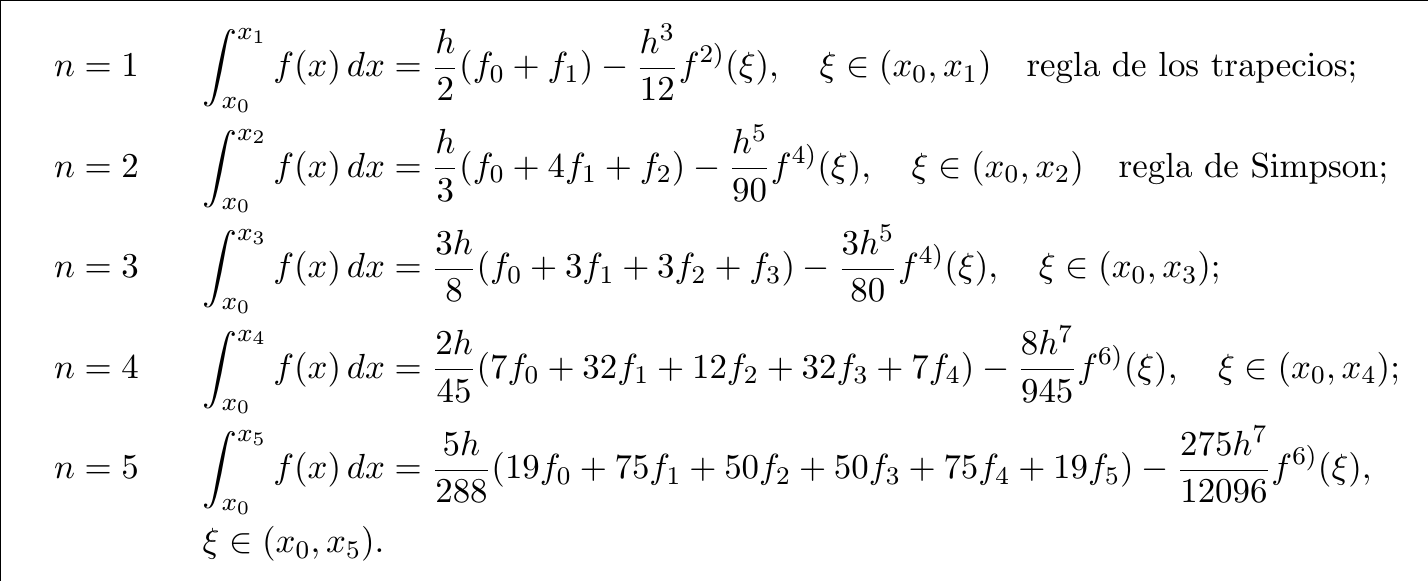
\includegraphics[width=0.95\linewidth]{tema3/formulas-nc-cerradas}
  \end{center}
\end{example}

\begin{example}[Fórmulas de cuadratura abiertas]
  \label{ex:fc-NC-abiertas}
  Sean $x_0,x_1,\cdots,x_n$ los $n+1$ puntos interiores al intervalo
  $[a,b]$ en una f.c. de N--C abierta. Denotemos ahora $x_{-1}=a$,
  $x_{n+1}=b$ y $f_k=f(x_k)$, $k=0,\dots,n$. Procediendo como antes
  se tienen las siguientes fórmulas junto con las expresiones de error
  asociadas:
  \begin{center}
    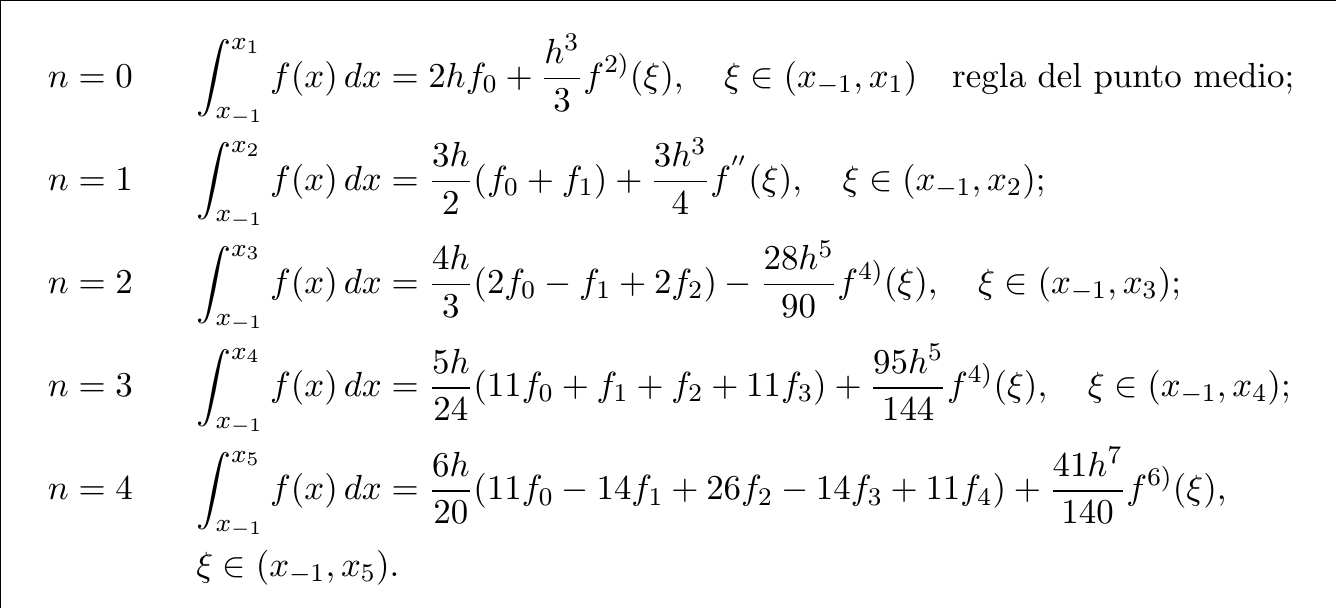
\includegraphics[width=0.95\linewidth]{tema3/formulas-nc-abiertas}
  \end{center}
  Se recomienda, como ejercicio, comprobar estas fórmulas para algunos
  valores de $n$.
\end{example}

\section{Fórmulas de cuadratura compuestas}
\label{sec:fc-compuestas}

A medida que aumenta el número de nodos en las f.c. de N-C, el número
de operaciones necesarias para el cálculo de los pesos comienza a ser
demasiado costoso. Y, lo que es más importante, no podemos asegurar
que, cuando $n\to\infty$, la aproximación $I_n(f)$ converja hacia la
integral de $f$ (de forma similar a lo que ocurre al
aumentar el grado en el polinomio de interpolación de Lagrange). Por
esta razón, en la práctica se usan fórmulas de cuadratura
compuestas (o integración a trozos).

Las fórmulas compuestas se definen de la siguiente forma: sea una
partición del intervalo $[a,b]$, $a=\ox_0<\ox_1<...<\ox_N=b$, que por
simplicidad supondremos uniforme (con $N+1$ puntos
equiespaciados).  Descomponemos
la integral global de $f$ como suma de integrales en cada subintervalo
$[\ox_{i-1},\ox_i]$:
\begin{equation*}
  \int_a^b f(x)\,dx = \sum_{i=1}^N \int_{\ox_{i-1}}^{\ox_i}f(x)\,dx.
\end{equation*}
A continuación aplicamos, en cada uno de estos subintervalos, una
fórmula de cuadratura sobre $n+1$ puntos, con $n\in\Nset$ fijo (en la
práctica se suelen usar fórmulas sencillas, en concreto fórmulas de
N--C con $n=0$, $1$ o $2$). Así, podemos aproximar la integral de $f$
haciendo que $h\to 0$, donde $h=(b-a)/N$ es la longitud de
los subintervalos.

Con más detalle: en el subintervalo $[\ox_{i-1},\ox_i]$ elegimos $n+1$
puntos equiespaciados, $\ox_0^{(i)}<\ox_1^{(i)}<\cdots<\ox_n^{(i)}$, y
consideramos una f.c:
\begin{align}
  \label{eq:fc.compuesta.en.un.intervalo}
  I_n^i(f)&=\sum_{j=0}^n \omega_j^{(i)}f(x_j^{(i)}),
\intertext{en la que el error viene dado (por definición) como:}
  E_n^i(f)&=\int_{\ox_{i-1}}^{\ox_i} f(x)\,dx -  I_n^i(f).
  \label{eq:fc.compuesta.error.subintervalos}
\end{align}
\begin{definition}
  Una fórmula de cuadratura compuesta se define como la suma de las
  f.c. en cada uno de los subintervalos de integración:
  \begin{equation*}
    I_N(f)=\sum_{i=1}^N I_n^i(f)  =\sum_{i=1}^N \sum_{j=0}^n \omega_j^{(i)}f(x_j^{(i)}).
  \end{equation*}
  \label{def:fc.compuesta}
\end{definition}
\subsection*{Expresión del error en fórmulas compuestas}
Si definimos el error de cuadratura en una fórmula compuesta como la
diferencia entre la integral $\int_a^b f(x)\,dx$ y su aproximación
$I_N(f)$, es fácil ver que este error coincide con la suma de los
errores en los $N$ subintervalos $[\ox_{i-1},\ox_i]$:
\begin{alignat*}{2}
  E_N(f)&= \int_a^b f(x)\,dx - I_N(f)  
  &\quad \text{(definición del error de integración)}
  \\
  &= \sum_{i=1}^N \int_{\ox_{i-1}}^{\ox_i} f(x)\,dx -
  \sum_{i=1}^NI_n^i(f) 
  &\text{(definición de una f.c. compuesta)}
  \\ 
  &= \sum_{i=1}^N\left(
    \int_{\ox_{i-1}}^{\ox_i} f(x)\,dx -  I_n^i(f) \right)
  =\sum_{i=1}^N E_n^i(f) 
  &\text{(def. error en subintervalos~(\ref{eq:fc.compuesta.error.subintervalos}))}.
\end{alignat*}

Si acotamos los errores $E_n^i(f)$ que aparecen en el sumatorio
anterior utilizando la cota genérica del error de
cuadratura~(\ref{eq:cota-error-fcti}), podemos obtener una primera
estimación del error de cuadratura $E_N(f)$ (esta tarea se deja como
ejercicio).

Pero en el caso habitual estaremos utilizando fórmulas de N--C en cada
subintervalo, es decir con nodos equiespaciados, y por tanto nos
encontraremos con una situación más favorable: podemos identificar los
errores $E_n^i(f)$ usando el teorema~\ref{thm:error.formulas-nc}, en
concreto la expresión~(\ref{eq:error-formulas-nc}), llegando al
siguiente resultado:

\begin{theorem}
  \label{thm:cota.error.fc.compuestas-nc}
  Sea $I_N$ una f.c. compuesta sobre una partición uniforme
  $a=\ox_0<\ox_1<...<\ox_N=b$. Supongamos que $I_n$ está definida por una
  fórmula de N--C de $n+1$ puntos en cada subintervalo
  $[\ox_{i-1},\ox_i]$.  Si $f\in C^k([a,b])$, donde $k=n+2$ si $n$ es par
  y $k=n+1$ si $n$ es impar, entonces existe $\xi\in(a,b)$ tal que:
  \begin{equation}
    \label{eq:error.fc.compuesta-NC}
   E_N(f)= \int_a^bf(x)\,dx - I_N(f)
   = C_n \, (b-a) \, h^{k} \, f^{k)}(\xi),
  \end{equation}
  donde $h=(b-a)/N$ y $C_n$ es una constante universal (independiente
  de $f$ y del intervalo $[a,b]$). En concreto:
  \begin{equation*}
  C_n=\left\{
    \begin{array}{cl}
      \displaystyle\frac{\gamma_n}{n^k\,k!} & \quad \text{ si la fórmula de N--C es
        cerrada},
      \\ \noalign{\medskip}
      \displaystyle\displaystyle\frac{\gamma_n}{(n+2)^k\,k!} &\quad \text{ si la fórmula
        de N-C es abierta},
    \end{array}
  \right.
\end{equation*}
  donde $\gamma_n$ son las constantes definidas en el
  teorema~\ref{thm:error.formulas-nc}.
\end{theorem}

\begin{proof}~
  Hemos visto que $E_n(f)=\sum_{i=1}^N E_n^i(f)$.
  Si utilizamos la expresión~(\ref{eq:error-formulas-nc}) para el
  error $E_n^i(f)$ en el intervalo $[\ox_{i-1},\ox_i]$ llegamos
  literalmente a:
  \begin{align*}
    E_N(f)&=\sum_{i=1}^N E_n^i(f) =\sum_{i=1}^N \gamma_n \widehat
    h^{k+1} \frac{f^{k)}(\xi_i)}{k!}  = \gamma_n \frac{\widehat
      h^{k+1}}{k!} \sum_{i=1}^Nf^{k)}(\xi_i),
  \end{align*}
  donde $\gamma_n$, $\widehat h$ y $k$ vienen dados en el
  teorema~\ref{thm:error.formulas-nc} y $\xi_i\in(\ox_{i-1},\ox_i)$.
  
  Veamos que 
  \begin{equation}
    \label{eq:fc.7}
    \text{$\exists \xi\in(a,b)$ tal que }
    f^{k)}(\xi)=\frac 1N \sum_{i=1}^Nf^{k)}(\xi_i).
  \end{equation}
  Como $f\in C^k([a,b])$, $f^{k)}$ es continua en $[a,b]$ y por lo
  tanto alcanza todos los valores entre su mínimo y su máximo. Sean
  $m_k=\min_{x\in[a,b]} f^{k)}(x)$ y $M_k=\max_{x\in[a,b]}
  f^{k)}(x)$. Entonces, como para todo $\xi_i$ se tiene que $m_k\le
  f^{k)}(\xi_i)\le M_k$, deducimos que
  $$
  m_k \le \frac 1N \sum_{i=1}^Nf^{k)}(\xi_i) \le M_k,
  $$
  luego se verifica~(\ref{eq:fc.7}). Por lo tanto:
  \begin{equation}
    \label{eq:fc.8}
    E_N(f) = \gamma_n \frac{\widehat
      h^{k+1}}{k!} N f^{k)}(\xi) =   \gamma_n \frac{\widehat
      h^{k+1}}{k!}\; \frac{b-a}{h} \,  f^{k)}(\xi)
  \end{equation}

  Para terminar, es fácil relacionar $\widehat h$ con $h$, en función
  del tipo de fórmula de N-C usada en los subintervalos
  $[\ox_{i-1},\ox_i]$. En concreto:
  \begin{align*}
    \intertext{\quad $\bullet$ Si la f.c. N--C es \emph{cerrada}:
      $\widehat h=(\ox_i-\ox_{i-1})/n=h/n$ y, usando~(\ref{eq:fc.8}),}
    E_N(f) &= \gamma_n \, (b-a)\, \frac{h^{k}}{n^k\,k!} \,
    f^{k)}(\xi).  
    \intertext{\quad $\bullet$ Si la
      f.c. N--C es \emph{abierta}: $\widehat
      h=(\ox_i-\ox_{i-1})/(n+2)=h/(n+2)$ luego} 
    E_N(f) &= \gamma_n
    \, (b-a) \, \frac{h^{k}}{(n+2)^k\,k!} \, f^{k)}(\xi).
  \end{align*}
  En cualquiera de los dos casos, si definimos $C_n$ como se
  indica en el enunciado del teorema, llegamos a~(\ref{eq:error.fc.compuesta-NC}).
\end{proof}

Algunas observaciones sobre el teorema anterior:
\begin{enumerate}
\item La expresión del error~(\ref{eq:error.fc.compuesta-NC}) nos
  indica que
  \begin{equation*}
    |E_n(f)| \le C_n (b-a) h^k \|f^{k)}\|_{\infty,a,b},
  \end{equation*}
  lo que
  garantiza la convergencia de $I_N(f)$ hacia $\int_a^b f(x)\, dx$
  cuando $h\to 0$ (o, equivalentemente, cuando $N=(b-a)/h \to\infty$).
\item Más aún, la cota anterior nos indica cuál es exactamente la
  velocidad de convergencia en una f.c. compuesta (definida por una
  fórmula de N-C):
  \begin{equation*}
      E_N(f)=O(h^{k}), \quad \text{cuando } h\to 0,
  \end{equation*}
  donde, donde $O(h^m)$ se define en~(\ref{eq:def.O(h^m)}) y, si la
  fórmula de N-C es elegida inteligentemente ($n$ par), $k=n+2$.
  Obsérvese que el error en una fórmula compuesta se rebaja un orden
  respecto a~(\ref{eq:error-formulas-nc}) (asimilando $\widehat h =
  h$, salvo constante), por acumulación de los errores locales
  (cometidos en los subintervalos).
\end{enumerate}

\begin{example}[Fórmula compuesta del punto medio]
  Consideramos la fórmula compuesta definida, en cada subintervalo,
  por la fórmula del punto medio (fórmula de N.C. abierta con $n=0$):
  \begin{equation*}
    \int_{\ox_{i}}^{\ox_{i+1}} f(x)\, dx \approx I_0(f)=
    (\ox_{i+1}-\ox_{i}) \, f\big(\frac{\ox_{i+1}+\ox_{i}} 2 \big), \quad i=0,...,N-1.
  \end{equation*}
  Para simplificar la notación en la f.c. compuesta, denotamos
  $$
  h=\hat h =\frac{\ox_{i+1}-\ox_{i}}{n+2}=\frac{\ox_{i+1}-\ox_{i}}2 =
  \frac{b-a}{2N},
  $$
  con lo que los puntos de integración (puntos medios) son de la
  forma $\ox_{i}+h$.
  Así, si definimos la partición $\{x_k\}_{k=0}^{2N}$ como
  \begin{equation*}
    \left\{
      \begin{aligned}
        x_{2i} &= \ox_i, \quad i=0,...,N \quad \text{(extremos de los
          intervalos)},
        \\
        x_{2i+1} &= x_{2i}+h \quad i=0,...,N-1
        \quad\text{(puntos medios)},
      \end{aligned}
      \right.
    \end{equation*}
  podemos utilizar, en cada subintervalo, la expresión de la f.c. del
  punto medio (véase el Ejemplo~\ref{ex:fc-NC-abiertas}) de donde:
  \begin{equation*}
    \int_{2x_i}^{2x_{i+2}} f(x)\, dx = 
    2hf_{2i+1} +
    \frac{h^3}{3}f^{''}(\xi_i), \quad \text{con }
    \xi_i\in(2x_i,2x_{i+2}),\ i=0,...,N-1
  \end{equation*}
  siendo $f_{2i+1}=f(x_{2i+1})$. En consecuencia:
  \begin{equation*}
    \int_a^b f(x)\,dx = \sum_{i=0}^{N-1} \int_{x_{2i}}^{x_{2i+2}} f(x)\,dx
    = 2h \sum_{i=0}^{N-1} f_{2i+1} + \frac{h^3}{3} \sum_{i=0}^{N-1}f''(\xi_i). 
  \end{equation*}
  Para terminar, agruparemos los términos de error en un único
  sumando. Para ello, procedemos como en la demostración del teorema
  anterior (en concreto, como en la demostración de~(\ref{eq:fc.7}), con
  $k=2$) y así deducimos que existe $\xi\in(a,b)$ tal que
  $$\sum_{i=0}^{N-1}f''(\xi_i)=Nf''(\xi)=\frac{b-a}{2h}f(\xi),$$
  obteniendo la expresión definitiva:
  \begin{equation*}
    \int_a^b f(x)\,dx 
    = 2h \sum_{i=0}^{N-1} f_{2i+1} + \frac{(b-a)h^2}{6} f''(\xi).
  \end{equation*}  
\end{example}

\begin{example} [Fórmula compuesta de Simpson]
  Consideramos ahora la fórmula compuesta definida, en cada
  subintervalo, $[\ox_{i},\ox_{i+1}]$, con $i=0,...,N-1$, como
   \begin{equation*}
    \int_{\ox_{i}}^{\ox_{i+1}} f(x)\, dx \approx I_1(f)=
    \frac{\ox_{i+1}-\ox_{i}}{6} \, \left[f(\ox_i) + 
      4f\left(\frac{\ox_{i}+\ox_{i+1}}{2}\right)+f(\ox_{i+1})\right].
  \end{equation*}
  Como ejercicio se puede comprobar que, procediendo como en el
  ejemplo anterior, se obtiene la siguiente expresión para la fórmula
  compuesta de Simpson:
  \begin{equation*}
    \int_a^b f(x)\,dx 
    = \frac{h}{3} \left[
      f_0 
      + 2\sum_{i=1}^{N-1} f_{2i} 
      + 4\sum_{i=0}^{N-1} f_{2i+1} 
      + f_{2N} \right]
    + \frac{(b-a)h^4}{180} f^{4)}(\xi).
  \end{equation*}  
\end{example}

\section{Fórmulas de cuadratura de Gauss}
\label{sec:fc-Gauss}
Dada una fórmula de cuadratura $I_n(f)=\sum_{i=0}^n \omega_i f(x_i)$,
donde $\{x_i\}$ son $n+1$ nodos distintos fijos en
$[a,b]$, en la sección~\ref{sec:cuadratura-interpolatorio} (en
concreto, en la Proposición~\ref{pro:existencia.fcti}) hemos visto que
podemos elegir $n+1$ pesos $\omega_i$ de forma adecuada (de hecho,
$\omega_i=\int_a^b L_i(x)\, dx$, es decir la fórmula debe ser de tipo
interpolatorio) para que la fórmula de cuadratura asociada tenga orden
máximo, es decir orden $\ge n$.

En la secciones~\ref{sec:formulas-de-newton}
y~\ref{sec:fc-compuestas}, dedicadas respectivamente a las f.c. de
Newton-Côtes y a las f.c. compuestas, nos hemos limitado a escoger
nodos equiespaciados (la elección más sencilla) pero sin que exista
ningún tipo de garantía de que ésta sea la elección óptima. En esta
sección nos preguntaremos si es posible elegir los nodos de manera
adecuada para que el orden de la f.c. sea el mayor posible. En
concreto, planteamos el siguiente problema:
\begin{equation}
\label{eq:pb.fc.Gauss}
\tag{P}
\left.
  \begin{aligned}
    &\text{Elegir el soporte $S=\{x_0<x_1<...<x_n\}\subset [a,b]$}
    \\
    &\text{tal que la f.c.t.i. asociada sea de orden máximo.}
  \end{aligned}
\right\}
\end{equation}

\begin{definition}
  Las fórmulas de cuadratura con pesos obtenidos como solución del
  problema~(\ref{eq:pb.fc.Gauss}) reciben el nombre de fórmulas de
  cuadratura de Gauss.
\end{definition}
\subsection*{Aproximación heurística}
Para resolver el problema anterior, intentemos razonar como en la
demostración de la proposición~\ref{pro:existencia.fcti} (en la que se
determinaron de forma óptima los coeficientes $\omega_i=\int_a^b
L_i(x)\, dx$ como solución de un sistema lineal de ecuaciones con
matriz de Vandermonde).


Una f.c. $I_n(f)=\sum_{i=0}^n \omega_i f(x_i)$ tiene orden $m\in\Nset$
si y solo si se verifican $m+1$ ecuaciones:
\begin{alignat*}{2}
  E_n(x^0)&=\int_a^b x^0\, dx -I_n(x^0)&\; =0 \\
  E_n(x^1)&=\int_a^b x^1\, dx -I_n(x^1)&\; =0 \\
  % E_n(x^2)&=\int_a^b x^2\, dx -I_n(x^2)&\; =0 \\
  &~\quad\vdots \\
  E_n(x^m)&=\int_a^b x^m\, dx -I_n(x^m)&\; =0
\end{alignat*}
En esta ocasión, en la f.c. podemos elegir los $n+1$ nodos
$\{x_i\}_{i=0}^n$ y los $n+1$ pesos, $\{\omega_i\}_{i=0}^n$. En total
tenemos a nuestra disposición $2n+2$ incógnitas, por tanto, para que
el sistema de ecuaciones anterior tenga matriz cuadrada, deberá estar
formado por $2n+2$ ecuaciones, es decir, debe ser $m=2n+1$. Esto
significa que podemos aspirar a que las fórmulas de cuadratura de
Gauss tengan orden $2n+1$.  El inconveniente es que en este caso, el
sistema de ecuaciones no es lineal por lo que, salvo en casos
sencillos, no será posible recurrir esta estrategia para calcular los
nodos de integración.

\begin{example}
  Dado el intervalo $[a,b]=[-1,1]$, buscamos dos puntos $x_0,x_1\in
  [a,b]$ y dos pesos $\omega_i\in\Rset$ tales que la f.c. asociada sea
  de orden $2n+1=3$. Para ello, imponemos que esta f.c. sea exacta
  para los polinomios $x^i$, $i=0,...,3$:
  \begin{alignat*}{3}
    E_n(x^0)&=\int_{-1}^1 x^0\, dx - I_n(x^0)\ =\ 0 \ \Leftrightarrow
    \quad & 2 &= \omega_0+\omega_1,\\
    E_n(x^1)&=\int_{-1}^1 x^1\, dx - I_n(x^1)\ =\ 0 \ \Leftrightarrow
    \quad & 0 &=  \omega_0x_0+\omega_1x_1,\\
    E_n(x^2)&=\int_{-1}^1 x^2\, dx - I_n(x^2)\ =\ 0 \ \Leftrightarrow
    \quad & \frac{2}{3} &= \omega_0x_0^2+\omega_1x_1^2,\\
    E_n(x^3)&=\int_{-1}^1 x^3\, dx - I_n(x^3)\ =\ 0 \ \Leftrightarrow
    \quad &0 &= 
    \omega_0x_0^3+\omega_1x_1^3.
  \end{alignat*}
  De la segunda y la cuarta ecuaciones deducimos que $x_0=+x_1$ ó
  $x_0=-x_1$ y $\omega_0=+\omega_1$ ó $\omega_0=-\omega_1$. Pero
  teniendo en cuenta la primera ecuación, la única posibilidad es
  $\omega_0=\omega_1=1$ y, según la tercera ecuación,
  $x_0=x_1=\frac{1}{\sqrt 3}$. Por lo tanto, la fórmula de cuadratura
  de Gauss con dos puntos en el intervalo $[-1,1]$ se puede expresar
  de la siguiente forma:
  \begin{equation*}
    \int_{-1}^1 f(x)\, dx \approx f\Big( \frac{-1}{\sqrt 3} \Big)
    + f\Big(\frac{1}{\sqrt 3}\Big).
  \end{equation*}
\end{example}

\subsection*{Polinomios ortogonales} 
En fórmulas de cuadratura de Gauss, en vez de la resolución de los
sistemas no lineales descritos anteriormente, calcularán los nodos
óptimos como raíces de unas familias de polinomios conocidos como
polinomios ortogonales.

\begin{definition}
  \label{def:pol-orgotonales}
  Consideremos el espacio vectorial $\Pol_n[x]$, formado por los
  polinomios de grado menor o igual que $n$. Una base
  $\{\phi_0,\phi_1,\dots,\phi_n\}$ de $\Pol_n[x]$ (donde cada $\phi_i$
  tiene grado exactamente igual a $n$) se dice ortogonal en
  $[a,b]$
  \begin{equation*}
    \int_a^b \phi_i(x) \phi_j(x)\, dx = 0 \quad \text{si } i\neq j.
  \end{equation*}
  Una base se dice ortonormal cuando es ortogonal y además los
  polinomios son unitarios, en el siguiente sentido:
  \begin{equation*}
    \int_a^b (\phi_i(x))^2 \,dx = 1.
  \end{equation*}
\end{definition}

\begin{proposition}
  Para todo $n\ge 0$ existen bases ortogonales,
  $\{\phi_0,\phi_1,\dots,\phi_n\}$, de $\Pol_n[x]$, que se pueden
  construir mediante el siguiente algoritmo, conocido como método de
  ortogonalización de Gram-Schmidt:
  \begin{quotation}
    Dada una base (no necesariamente ortogonal),
    $\{\varphi_0,\varphi_1,\dots,\varphi_n\}$ de $\Pol_n[x]$,
    definimos
    \begin{align*}
      \phi_0 &= \varphi_0,\\
      \phi_1 &= \varphi_1 -
      \frac{\int_a^b\phi_0\varphi_1}{\int_a^b\phi_0^2} \phi_0\\
      &\ \vdots\\
      \phi_n &= \varphi_n -
      \frac{\int_a^b\phi_{n-1}\varphi_n}{\int_a^b\phi_{n-1}^2} \phi_{n-1}\\
    \end{align*}
  \end{quotation}
\end{proposition}

\begin{proof}
  Es fácil comprobar que el conjunto $\{\phi_0,\phi_1,\dots,\phi_n\}$
  construido mediante el método de Gram-Schmidt es ortogonal.
\end{proof}

\begin{proposition}
  Dadas dos bases ortogonales de $\Pol_n[k]$,
  $\{\phi_0,\phi_1,\dots,\phi_n\}$ y
  $\{\overline\phi_0,\overline\phi_1,\dots,\overline\phi_n\}$ los
  polinomios de cada una de estas bases son proporcionales, es decir,
  para cada $i=0,...n$ existe $\alpha_i$ tal que
  \begin{equation*}
    \phi_i = \alpha_i ,\overline\phi_i.
  \end{equation*}
  En particular, $\phi_i$ y $\overline\phi_i$ tienen los mismos
  ceros.
\end{proposition}

\begin{theorem}
  Sea $\{\phi_0,\phi_1,\dots,\phi_n\}$ un conjunto de polinomios
  ortogonales en $[a,b]$. Entonces cada polinomio $\phi_k$ tiene
  exactamente $k$ raíces reales simples $\{x_0<x_1<...<x_k\}$ en
  $(a,b)$.
\end{theorem}

\begin{theorem}
  Existe una única f.c.t.i. de orden $(2n+1)$. Esta fórmula se
  corresponde con el soporte $S=\{x_0<x_1<...<x_n\}$ formado por las
  $n+1$ raíces de $\phi_{n+1}$, el $n$--ésimo polinomio ortogonal en
  $(a,b)$. Además, los pesos $\omega_i=\int_a^b L_i(x)\, dx$ son todos
  positivos.
\end{theorem}
%%% Local Variables:
%%% mode: latex
%%% TeX-master: "../apuntes-MNII.tex"
%%% End: 
